\section{BGPmon: New Monitoring System}
\label{sec:main}

Open source routing software that is currently used as a collector typically implements a full routing protocol, including receiving routes, applying policies, setting forwarding states, and announcing routes to peers. 
These activities involve considerable complexity, but none of these actions are needed to be collector. 
A collector simply needs to receive and log routes. 
Our new collector design focuses on a narrow set of data collection functions. 
By focusing on the collection functionality and eliminating unnecessary tasks, the new collector is able to scale up and support more peer routers while making the data available in real-time to a potentially vast number of clients. 

%\begin{figure*}[t]
%\centering
%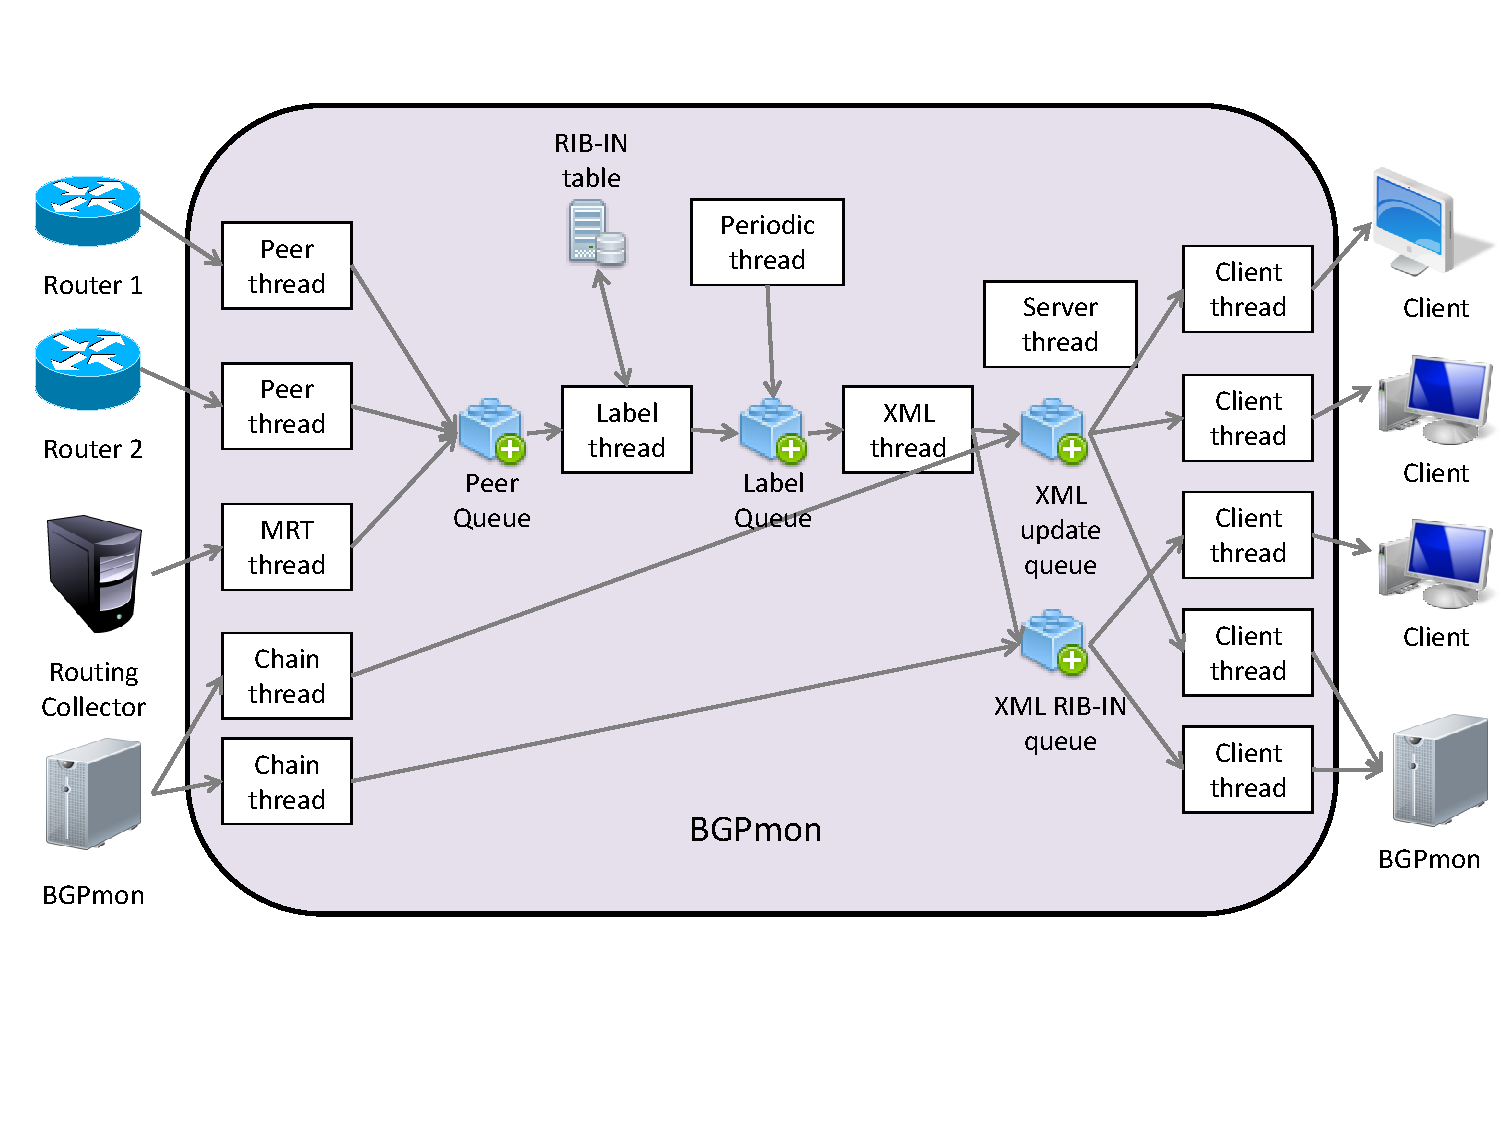
\includegraphics[scale=0.50]{figs/BGPmon-architecture.pdf}
%\caption{BGPmon architecture.}
%\label{architecturediagram}
%\end{figure*}

To support hundreds of peer routers and clients, one would like to scale out across multiple systems by adding more collectors and distributing the services. 
At the same time, a client should see a single monitoring service and be unaware that the implementation of the service may be done through multiple collectors. 
Our approach is based on publish/subscribe overlay networks that consist of brokers, publishers, and subscribers. 
The brokers form the overlay network, allowing publishers to send event streams to the overlay network and allowing subscribers to receive event streams from the overlay network. 
Publishers and subscribers interact only with brokers, not with each other, allowing the overlay network to insulate publishers and subscribers from each other. 

To improve fault tolerance, multiple brokers may monitor the same or different peers in an AS, yet appear to a client application as a single subscription. 
This allows critical applications to continue to receive event streams in the case of a failure of a peer, monitor, or broker. 
Our system implementation begins with BGPmon, a simple monitoring system now available that incorporates all three functions: publish, broker, and subscribe. 

